\documentclass[14pt]{article}
\usepackage[utf8]{inputenc}
\usepackage{listingsutf8}
%\usepackage[T2A]{fontenc}
\usepackage[english]{babel}
\usepackage{amssymb,amsmath,amsfonts,amsbsy}
%\usepackage{mathtext}
%\usepackage{indentfirst}
\usepackage{tabularx}
\usepackage{booktabs}
\usepackage{graphicx}
\usepackage[center]{caption}
\captionsetup{justification=raggedright,singlelinecheck=false}
\usepackage{subcaption}
\usepackage{cite}
\usepackage{enumerate}
\usepackage{enumitem}
%%\usepackage[braket]{qcircuit}
\usepackage{marvosym}
\usepackage{multicol}
\usepackage{comment}
\usepackage{authblk}
\usepackage{lipsum}
%\usepackage{hyperref}
\graphicspath{{figs/}}
%\DeclareGraphicsExtensions{.pdf,.png,.jpg}
%\bibliographystyle{utf8gost780u}
%\usepackage{apacite}
%\bibliographystyle{apacite}

% Print line number page wisely 
%\usepackage[pagewise]{lineno}
%\linenumbers

%\renewcommand\linenumberfont{\normalfont\bfseries\normal}
%\renewcommand\linenumberfont{\normal}

\title{\textbf{Schizophrenia Detection from MR images}}

%\author[1]{Ilia Golub}
\author[]{Ilia Golub}

%\author[1]{Pratit Kandel}

%\author[1]{Prosperity Oguama}
\author[]{Prosperity Oguama}


%\affil[1]{Gonda Multidisciplinary Brain Research Center, Bar-Ilan University, Ramat Gan, Israel}
\affil[]{Gonda Multidisciplinary Brain Research Center, Bar-Ilan University, Ramat Gan, Israel}
%\affil[4]{Institute of Natural Sciences and Mathematics, Ural Federal University, Ekaterinburg, Russia}
%\affil[5]{Department of Cardiology, Clinical Sciences, Lund University, Lund, Sweden}
%\affil[6]{Arrhythmia Clinic, Skane University Hospital, Lund, Sweden}
%\affil[*]{Correspondence: golub.ilia.ilya@gmail.com}

\setcounter{Maxaffil}{0}
\renewcommand\Affilfont{\itshape\small}
\date{}

\usepackage[onehalfspacing]{setspace}

\usepackage{listings}
\renewcommand{\lstlistingname}{Listing}
\lstset{language=Python,
        numbers=left,
        basicstyle=\small\ttfamily,
        breaklines=true,
        showstringspaces=false,
        stepnumber=1,         
        numbersep=5pt,          
        showspaces=false,       
        showtabs=false,         
        %frame=single,          
        tabsize=4,              
        captionpos=b,           
        breakatwhitespace=false,
        escapeinside={\%*}{*)}, 
        texcl=true
        }

\usepackage[left=2.5cm, right=1cm, top=1cm, bottom=2.5cm]{geometry}

\usepackage[
    colorlinks=true,
    linkcolor=blue,
    filecolor=magenta,      
    urlcolor=cyan,
    pdftitle={CW-2},
    pdfauthor={Golub I},
    bookmarks=true,
    linktoc=all,
	final]{hyperref}

\usepackage[nottoc]{tocbibind}

\makeatletter
\renewcommand{\@biblabel}[1]{#1.}
\makeatother

\sloppy

\righthyphenmin=2

\renewcommand{\theenumi}{\arabic{enumi}.}
\renewcommand{\labelenumi}{\arabic{enumi}.} 
\renewcommand{\theenumii}{\arabic{enumii}.} 
\renewcommand{\labelenumii}{\arabic{enumi}.\arabic{enumii}.}
\renewcommand{\theenumiii}{\arabic{enumiii}.} 
\renewcommand{\labelenumiii}{\arabic{enumi}.\arabic{enumii}.\arabic{enumiii}.} 


\DeclareMathOperator{\rot}{rot}		% Определяем операции rot
\DeclareMathOperator{\diverg}{div}	% div
\DeclareMathOperator{\grad}{grad}	% grad
\DeclareMathOperator{\arth}{Arth}    % arc tanh
\DeclareMathOperator{\Ai}{Ai}
\DeclareMathOperator{\Bi}{Bi}

\setcounter{tocdepth}{1}

\begin{document}

% Title
\maketitle

% Abstract
\section{Abstract}

\textbf{Background}\\
Schizophrenia (SZ) is a chronic mental disorder that presents challenges in accurate diagnosis due to its complex nature. Advances in machine learning (ML) and deep learning (DL) have shown promise in automating SZ detection using structural MRI, but variability in preprocessing methods remains a key challenge.
\textbf{Aim}: This study aims to evaluate the impact of various preprocessing and data augmentation techniques on ML-based classification of schizophrenia from MRI data.

\textbf{Methods}\\
We utilized a subset of the COBRE dataset, which includes structural MRI data from 62 individuals, divided into 30 schizophrenia patients and 32 healthy controls. A support vector classifier (SVC) was employed to classify the images. Various preprocessing techniques --- resampling, normalization, brain extraction, cropping, smoothing --- and data augmentation methods -- translation, rotation, and Gaussian noise addition --- were applied to the MRI data. Model performance was assessed using accuracy, recall, precision, and F1-score.

\textbf{Results}\\
Normalization and brain extraction improved classification accuracy, with cropping achieving the highest accuracy (57\%) and F1-score (0.69) among the preprocessing techniques. Combining preprocessing methods did not always result in performance improvements and sometimes led to a decrease in accuracy. The combination of resampling, normalization, and brain extraction gave the best performance (accuracy of 55\% and F1-score of 0.69) among the combinations explored in this study. Data augmentation significantly enhanced model performance, with translation and rotation leading to the highest accuracy (0.79) and F1-score (0.80). The data for the final model was preprocessed with the optimal combination, translated, and rotated at random (resampling + normalization + brain extraction + translation + rotation) and produced the highest recorded accuracy and recall scores (81\% and 0.98 respectively).

\textbf{Conclusion}\\
Our findings indicate that careful selection of preprocessing and augmentation techniques is critical for optimizing model performance in schizophrenia detection. While certain preprocessing steps like cropping and smoothing are beneficial, combining them may not always yield additive improvements. Augmentation techniques like translation and rotation proved effective in boosting model performance, due to their ability to increase the data size. These results contribute to the development of more standardized preprocessing pipelines for medical imaging, which could enhance the reliability and reproducibility of machine learning models in clinical applications.

\textbf{Keywords: schizophrenia, sMRI, CNN, SVC}

% Introduction
\section{Introduction}

Schizophrenia (SZ) is a chronic mental disorder affecting 1 in 300 people worldwide, linked to structural brain abnormalities observable via MRI. Machine learning (ML) and deep learning (DL) have advanced SZ diagnosis, yet variability in preprocessing methods—such as noise removal and intensity normalization—remains a major challenge~\cite{Benli2023, Zhang2022}.

Despite progress in CNN-based SZ detection, studies often lack standardized preprocessing pipelines, impacting model reliability and reproducibility. Benchmark datasets~\cite{Oh2020, Verma2023} report high classification accuracies, but inconsistent preprocessing limits comparability.

This study systematically evaluates preprocessing and augmentation techniques to establish a robust pipeline for SZ detection from MRI. Standardizing these practices could improve the reproducibility and clinical applicability of ML-based diagnostics.

% Methods
\section{Methods}

\subsection{Dataset and Exploratory Data Analysis}

The raw data were obtained from the \href{http://schizconnect.org}{SchizConnect} database (accessed January 1, 2025), which houses structural and functional MRI data. The database provides filtering options to enable users to select data that meets specific criteria including MRI field strength and clinical diagnosis (e.g. schizophrenia, bipolar disorder).

The data obtained originates from the Center of Biomedical Research Excellence (COBRE) dataset in NifTI format. It includes data from 62 individuals, 30 with schizophrenia and 32 healthy controls.

The data from SchizConnect was filtered based on MRI field strength and clinical diagnosis. We retrieved only images captured with 3T MRI scans. This was done to ensure uniformity of the data obtained. Figure~\ref{fig:raw_mri_volume_slices} presents the example of raw data.
\begin{figure}[h]
    \centering
    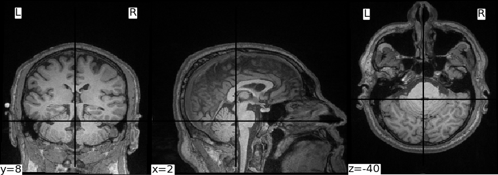
\includegraphics[width=0.8\textwidth]{./figs/sample_volume.png} %
    \caption{Three image slices representing the average of a 3D column in three views: dorsal, lateral, and superior respectively}\label{fig:raw_mri_volume_slices}
\end{figure}

Clinical data was made available in form of CSV files. The demographic features of the dataset used in this project are presented in Table~\ref{tab:cobre_clinical_demographic}.
\begin{center}
	\begin{table}
        \centering
        \caption{\label{tab:cobre_clinical_demographic}The subjects were selected to give a balanced representation of age and gender distributions in the dataset, prioritizing age distribution, which has been shown to affect model performance ~\cite{Oh2020}.}
        \begin{tabular*}{500pt}{@{\extracolsep\fill}lcccccc@{\extracolsep\fill}}
            \toprule
            & \multicolumn{3}{c}{COBRE}
            \\\cmidrule{2-4}
            & \textbf{Individuals with SZ (n=30)} & \textbf{Healthy controls (n=32)} & \textbf{Total (62)} \\
            \midrule
            Minimum age             & 19  & 18  & 18 \\
            Maximum age 		    & 66  & 65 & 66  \\
            Average age             & 39.6 & 41 & 40.3	\\
            Gender (Male/ Female)   & 19/11 & 17/15 & 36/26	\\
            \bottomrule
        \end{tabular*}
    \end{table}    
\end{center}

%
\subsection{Image Preprocessing}

% General thoughts
The major idea behind preprocessing was to establish a standardized pipeline that ensures consistency in the quality and content of the MRI data. This pipeline addressed common issues such as noise, intensity variations, and artifacts, which can affect the performance of machine learning models.

We experimented with different preprocessing and data augmentation techniques, and their combinations, to determine which pipeline yields the best performance of the feature extraction model and a classifier regarding accuracy, recall rate, precision, and F1 score.

In order to find the best combination of hyperparameters for each preprocessing method, we performed a grid search and measured the quality metrics of the processed image using a custom test function.

Table~\ref{tab:preprocessing_pipeline} presents the preprocessing techniques used and their respective hyperparameters and tools used. Figure~\ref{fig:slice_comparison} gives a comparison of a raw image and a preprocessed image, also indicating the image metrics.
%Figure~\ref{fig:test_pipeline} gives a visual representation of the conducted tests.
%
\begin{figure}[h]
    \centering
    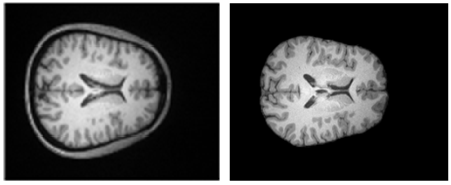
\includegraphics[width=0.6\textwidth]{./figs/slice_comparison.png} % test_pipeline.png
    \caption{Panel A shows a slice of a raw scan. Panel B shows a slice of a preprocessed scan. For preprocessed scans, the standard deviation of SNR values is relatively low (\mbox{$SNR= 25 \pm 1$}), which ensures consistency in the image quality and prevents the model from making predictions based on possible artifacts.}\label{fig:slice_comparison}
\end{figure}

\subsubsection{Resampling}

The first preprocessing technique employed was resampling the images to a standard resolution to ensure uniform input for the model and consistent noise and signal profiles.

\subsubsection{Intensity normalization}

The second technique normalization of voxel intensities to a consistent range to maintain the relative scale of the data and produce values in a fixed range to satisfy models expectations. The adopted method scales the data to a range of [0, 1].

Normalization also improves the results of brain extraction by helping the algorithm better distinguish between brain and non-brain regions.

Intensity distributions were inspected to ensure normalization did not distort the data.

\subsubsection{Brain extraction}

The third technique employed was a brain extraction. The purpose of this stage is to
\begin{itemize}
    \item remove non-brain regions in order to minimize noise, making it easier for the network to focus on relevant features;
    \item subsequently enhance the network's performance, especially in a schizophrenia detection task where small differences in brain anatomy are crucial;
    \item ensure that the input images are more consistent in terms of content, which can help the model generalize better.
\end{itemize}

The generated brain mask was refined by closing gaps and removing small regions. The mask was also used as a leverage for the cropping step.

\subsubsection{Cropping}

The fourth technique was cropping the brain region to a consistent size across scans.

\subsubsection{Smoothing}

The fifth technique was smoothing the brain region to reduce noise and variability introduced by acquisition artifacts, enhancing the overall quality of the images. This was done to ensure that the downstream tasks are more robust and the model training is more effective. We used a Gaussian filter to reduce high-frequency noise while preserving edges to some extent. Since the neural network performed a classification task, moderate smoothing was carried out to focus on broader patterns.

The sixth technique was normalization of the smoothed image to address potential intensity changes and ensure that all images are on a comparable scale.

\subsubsection{Validation}

The impact of preprocessing on the data's integrity and quality was assessed using a combination of a visual inspection and quantitative metrics. The visual inspection involved plotting a few slices of the MRI before and after each preprocessing step. Validation was performed to ensure that preprocessing steps did not introduce artifacts or distort anatomical structures, and to ensure consistency of the processed images.

Quantitative metrics included Signal-to-Noise Ratio (SNR), Contrast-to-Noise Ratio (CNR), Peak Signal-to-Noise Ratio (PSNR), and 
Structural Similarity Index (SSIM). 

Relative PSNR for one image. Using a hypothetical "ideal" signal (the maximum intensity value as a baseline), a relative PSNR for one image was calculated. This relative PSNR was used as a way to assess the "quality" of a single image compared to a theoretical perfect image of uniform intensity.

A binary mask was computed using Otsu's thresholding to explicitly select a background region for noise estimation.

The metrics were computed for the entire 3D volume to assess the overall quality or similarity of the entire MRI dataset, capturing global differences.
\begin{center}
    \begin{table}
        \centering
        \caption{\label{tab:preprocessing_pipeline}Preprocessing techniques and the corresponding parameters used in the study.}
        \begin{tabular*}{500pt}{@{\extracolsep\fill}lcc@{\extracolsep\fill}}
            \toprule
            \textbf{Preprocessing Step} & \textbf{Hyperparameters} & \textbf{Tools} \\
            \midrule
            Resampling & Voxel size: \texttt{2x2x2} & Nibabel library \\
            Intensity Normalization & Min-max scaling: [0, 1] & NumPy \\
            Brain Extraction & Modality: T1, U-net & ANTsPyNet \\
            Cropping & Size: based on the largest bounding box among all images & scikit-image, NumPy \\
            Smoothing & Gaussian filter: sigma=0.5 & SciPy \\
            \bottomrule
            \end{tabular*}
    \end{table}
\end{center}
%
\subsection{Data Augmentation}

According to typical variations in brain MRI scans, the following transformations with corresponding parameters were applied to the images:
\begin{itemize}
    %\item[\textbf{Option 1}]  \textbf{Shearing.} A shearing angle is selected randomly within the range $\left[-15^{\circ}, 15^{\circ}\right]$ and A shearing operation is applied within the x and y-axis. This operation is repeated 10 times with 10 different shearing angles. By this method, 10 images are generated from an original image;
    \item[\textbf{Option 1}] \textbf{Translation}. The operation is applied on the x and y-axis and repeated 10 times by using different values sampled randomly within the range $\left[-10, 10\right]$. By this method, 10 images are generated from an original image.
    \item[\textbf{Option 2}] \textbf{Rotation.} Rotation angles are selected randomly within the range  $\left[-10^{\circ}, 10^{\circ}\right]$ and clockwise rotations are applied using 10 different angle values. 10 images are generated from an original image by this method.
    \item[\textbf{Option 3}] \textbf{Gaussian noise addition.} Noise addition is applied by \mbox{$I=I+R*I*std+mean$}, where $I$ refers to the image, $R$ refers to the Noise. The noise to be added is generated using a Gaussian distribution. The variance of the distribution is computed from the input images while the mean value is set to zero. In this study, three different fixed values (0.1, 0.2, and 0.3) are used and 3 images are generated from an input image.
    %\item[\textbf{Option 4}] \textbf{Gaussian noise addition followed by rotation.} 30 images are generated from an input image by this method.
    %\item[\textbf{Option 5}] \textbf{Clockwise rotation followed by translation.} Rotation angles are selected randomly within the range $\left[-25^{\circ}, 25^{\circ}\right]$ and translation is applied on the x and y-axis by using different values sampled randomly within the range $\left[-15^{\circ}, 15^{\circ}\right]$. This successive operation is applied 10 times, and 10 images are generated from an input image by this method.
    %\item[\textbf{Option 6}] \textbf{Translation followed by shearing.} The translation step is applied on the x and y-axis with different values sampled randomly within the range $\left[-15, 15\right]$. In the shearing step, an angle is selected randomly within the range $\left[-15^{\circ}, 15^{\circ}\right]$, and shearing is applied within the x and y-axis. The subsequent operations are applied 10 times, and 10 images are generated from an input image by this method.
    %\item[\textbf{Option 7}] \textbf{Translation, shearing, and rotation.} Operations are applied subsequently. Implementation of the translation and shearing operations are performed as explained in the previous method. In the rotation step, a random angle is selected within the range $\left[-25^{\circ}, 25^{\circ}\right]$ clockwise rotation is applied. The successive operations are applied 10 times, and 10 images are generated from an input image by this method.
\end{itemize}

The augmented samples were plotted to ensure the transformations did not distort anatomical features.

%
\subsection{Model architectures}

Convolutional Neural Networks (CNNs) are commonly used in the literature for this task. However, a few papers explored the use of support vector machines for image classification. To gain a full understanding of both approaches, we decided on the combination of a pretrained deep neural network for feature extraction and a support vector classifier for binary classification. The ReNet-18 architecture was selected for its balance between computational load and accuracy. Cross validation was performed with the support vector classifier (SVC) to choose the best hyperparameters, and the hyperparameters that yielded the best results were the radial basis function (RBF) kernel, a gamma value of 0.0001 and a C parameter value of 100. Each 2D slice of the images were fed into the ResNet-18 model as NumPy arrays of dimension \texttt{224x224}. This input size corresponds to the size of the images in the ImageNet dataset that was used to train ResNet-18 and was selected for compatibility with the pretrained weights of the ResNet-18 model. Figure~\ref{fig:model_architecture} gives a representation of the training architecture and flow.
%
\begin{figure}
    \centering
    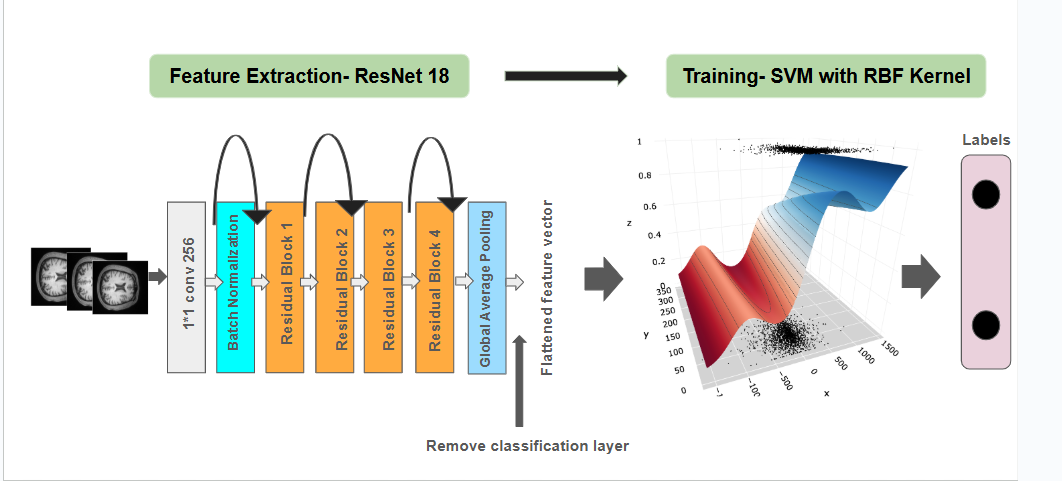
\includegraphics[width=0.8\textwidth]{./figs/model_architecture.png} %
    \caption{Overview of the training pipeline. Raw or preprocessed MRI slices are fed into a ResNet-18 model for feature extraction, where convolutional layers, batch normalization, and residual blocks process the input. The final feature vector, obtained after global average pooling and flattening, is passed to an SVM classifier with an RBF kernel for binary classification into schizophrenic and non-schizophrenic labels.}\label{fig:model_architecture}
\end{figure}

%
\subsection{Training and validation}

The dataset was split into a training set (80\%) and a validation set (20\%). 

Accuracy, recall, precision, and F1-score were calculated to asses the performance of the SVC.

% Results
\section{Results}

\subsection{Image Preprocessing}

The results presented in Table~\ref{tab:model_metrics_preprocessing} demonstrate the impact of various preprocessing methods on classification performance. The baseline model using raw images (0) achieved an accuracy of 51\%, with an F1-score of 0.63. Applying resampling (1) alone did not alter these results, suggesting that resampling alone does not introduce substantial benefits.

Normalization (2) improved accuracy to 56\% and F1-score to 0.67, indicating that standardizing intensity values enhances model performance. Brain extraction (3) yielded a slightly lower accuracy (54\%) but a notable increase in recall (0.78), which suggests that removing non-brain tissues helps capture more positive instances but may introduce a trade-off in precision.

Cropping (4) led to the highest accuracy (57\%) and an F1-score of 0.69, highlighting its effectiveness in improving signal-to-noise ratio. Smoothing (5) showed a moderate impact, improving results compared to the raw data but not outperforming other methods.

When combining preprocessing techniques, the pattern is less straightforward. The combination of resampling, normalization, and brain extraction (1+2+3) resulted in the highest recall (0.80) while maintaining a strong F1-score (0.69). However, adding cropping (1+2+3+4) caused a drastic performance drop, with accuracy declining to 44\% and F1-score to 0.54. The full pipeline (1+2+3+4+5) slightly improved over this but still underperformed compared to individual preprocessing steps.
\begin{center}
	\begin{table}[t]
		\centering
		\caption{\label{tab:model_metrics_preprocessing}Classification performance metrics for different preprocessing methods. Accuracy, recall, precision, and F1-score are reported for models trained on raw MRI slices and various preprocessing techniques. While normalization (2) and cropping (4) provided the highest accuracy (57\%), brain extraction (3) led to the highest recall (0.78). The combination of resampling, normalization, and brain extraction (1+2+3) resulted in the best recall (0.80) with a strong F1-score (0.69). However, adding cropping (1+2+3+4) and smoothing (1+2+3+4+5) led to performance degradation, suggesting that excessive preprocessing may reduce classification effectiveness.}
		\begin{tabular*}{500pt}{@{\extracolsep\fill}lcccc@{\extracolsep\fill}}
			\toprule
		     \textbf{Preprocessing method} &\textbf{Accuracy (\%)} &  \textbf{Recall} &\textbf{Precision} &\textbf{F1-score}\\
			\midrule
			Raw (0) & 51\% & 0.67 & 0.60 & 0.63 \\
			Resampling (1) & 51\% & 0.67 & 0.60 & 0.63 \\
			Normalization (2) & 56\% & 0.69 & 0.64 & 0.67 \\
			Brain extraction (3) & 54\% & 0.78 & 0.60 & 0.68 \\
			Cropping (4) & 57\% & 0.76 & 0.63 & 0.69 \\
			Smoothing (5) & 55\% & 0.71 & 0.62 & 0.66 \\
            1+2 & 57\% & 0.69 & 0.64 & 0.67 \\
            1+2+3 & 55\% & 0.80 & 0.61 & 0.69 \\
            1+2+3+4 & 44\% & 0.53 & 0.56 & 0.54 \\
            1+2+3+4+5 & 48\% & 0.60 & 0.58 & 0.59 \\
			\bottomrule
		\end{tabular*}
	\end{table}
\end{center}

\subsection{Data Augmentation}

The results presented in Table~\ref{tab:model_meetrics_augmentation} highlight the impact of various data augmentation methods on model performance. The baseline model using raw data (0) achieved an accuracy of 0.51 and an F1-score of 0.63. In contrast, applying translation (6) significantly improved both accuracy (75\%) and F1-score (0.79), with a notable increase in recall (0.84), indicating that translation is effective at boosting model performance and sensitivity.

Rotation (7) further improved results, with the highest accuracy (79\%) and F1-score (0.80), alongside strong recall (0.81) and precision (0.78), demonstrating its ability to enhance both model robustness and overall performance.

Gaussian noise (8), however, led to a substantial decrease in performance, with an accuracy of only 33\% and a low F1-score of 0.40. This suggests that adding noise may negatively affect the model, potentially obscuring relevant patterns in the data.
\begin{center}
	\begin{table}[t]
		\centering
		\caption{\label{tab:model_meetrics_augmentation}Classification performance metrics for different data augmentation methods. Accuracy, recall, precision, and F1-score are reported for models trained on raw MRI slices and augmented datasets. Both translation (6) and rotation (7) significantly improved model performance, with rotation achieving the highest accuracy (79\%) and F1-score (0.80). In contrast, Gaussian noise (8) led to a severe drop in performance, reducing accuracy to 33\% and F1-score to 0.40. The final training setup, combining preprocessing with translation and rotation (1+2+3+6+7), achieved the best overall results, with 81\% accuracy and the highest recall (0.98), indicating the effectiveness of spatial transformations in improving classification.}
		\begin{tabular*}{500pt}{@{\extracolsep\fill}lcccc@{\extracolsep\fill}}
			\toprule
			\textbf{Augmentation method} &\textbf{Accuracy (\%)} &  \textbf{Recall} &\textbf{Precision} &\textbf{F1-score}\\
			\midrule
			Raw (0) & 0.51 & 0.67 & 0.60 & 0.63 \\
			Translation (6) & 75\% & 0.84 & 0.74 & 0.79 \\
			Rotation (7) & 79\% & 0.81 & 0.78 & 0.80 \\
			Gaussian Noise (8) & 33\% & 0.32 & 0.53 & 0.40 \\
            Final training (1+2+3+6+7) & 81\% & 0.98 & 0.77 & 0.86 \\
			\bottomrule
		\end{tabular*}
	\end{table}
\end{center}

The final training combined the optimal combination of preprocessing with translation and rotation techniques (1+2+3+6+7), surpassing the accuracy and recall of all the experiments (81\% and 0.98 respectively), with a precision value only surpassed by the rotation experiment. Figure~\ref{fig:eval_final_model} shows the output of the final training and Figure~\ref{fig:model_metrics_comparison} shows the comparison between the metrics of all the preprocessing and augmentation experiments.
\begin{figure}
    \centering
    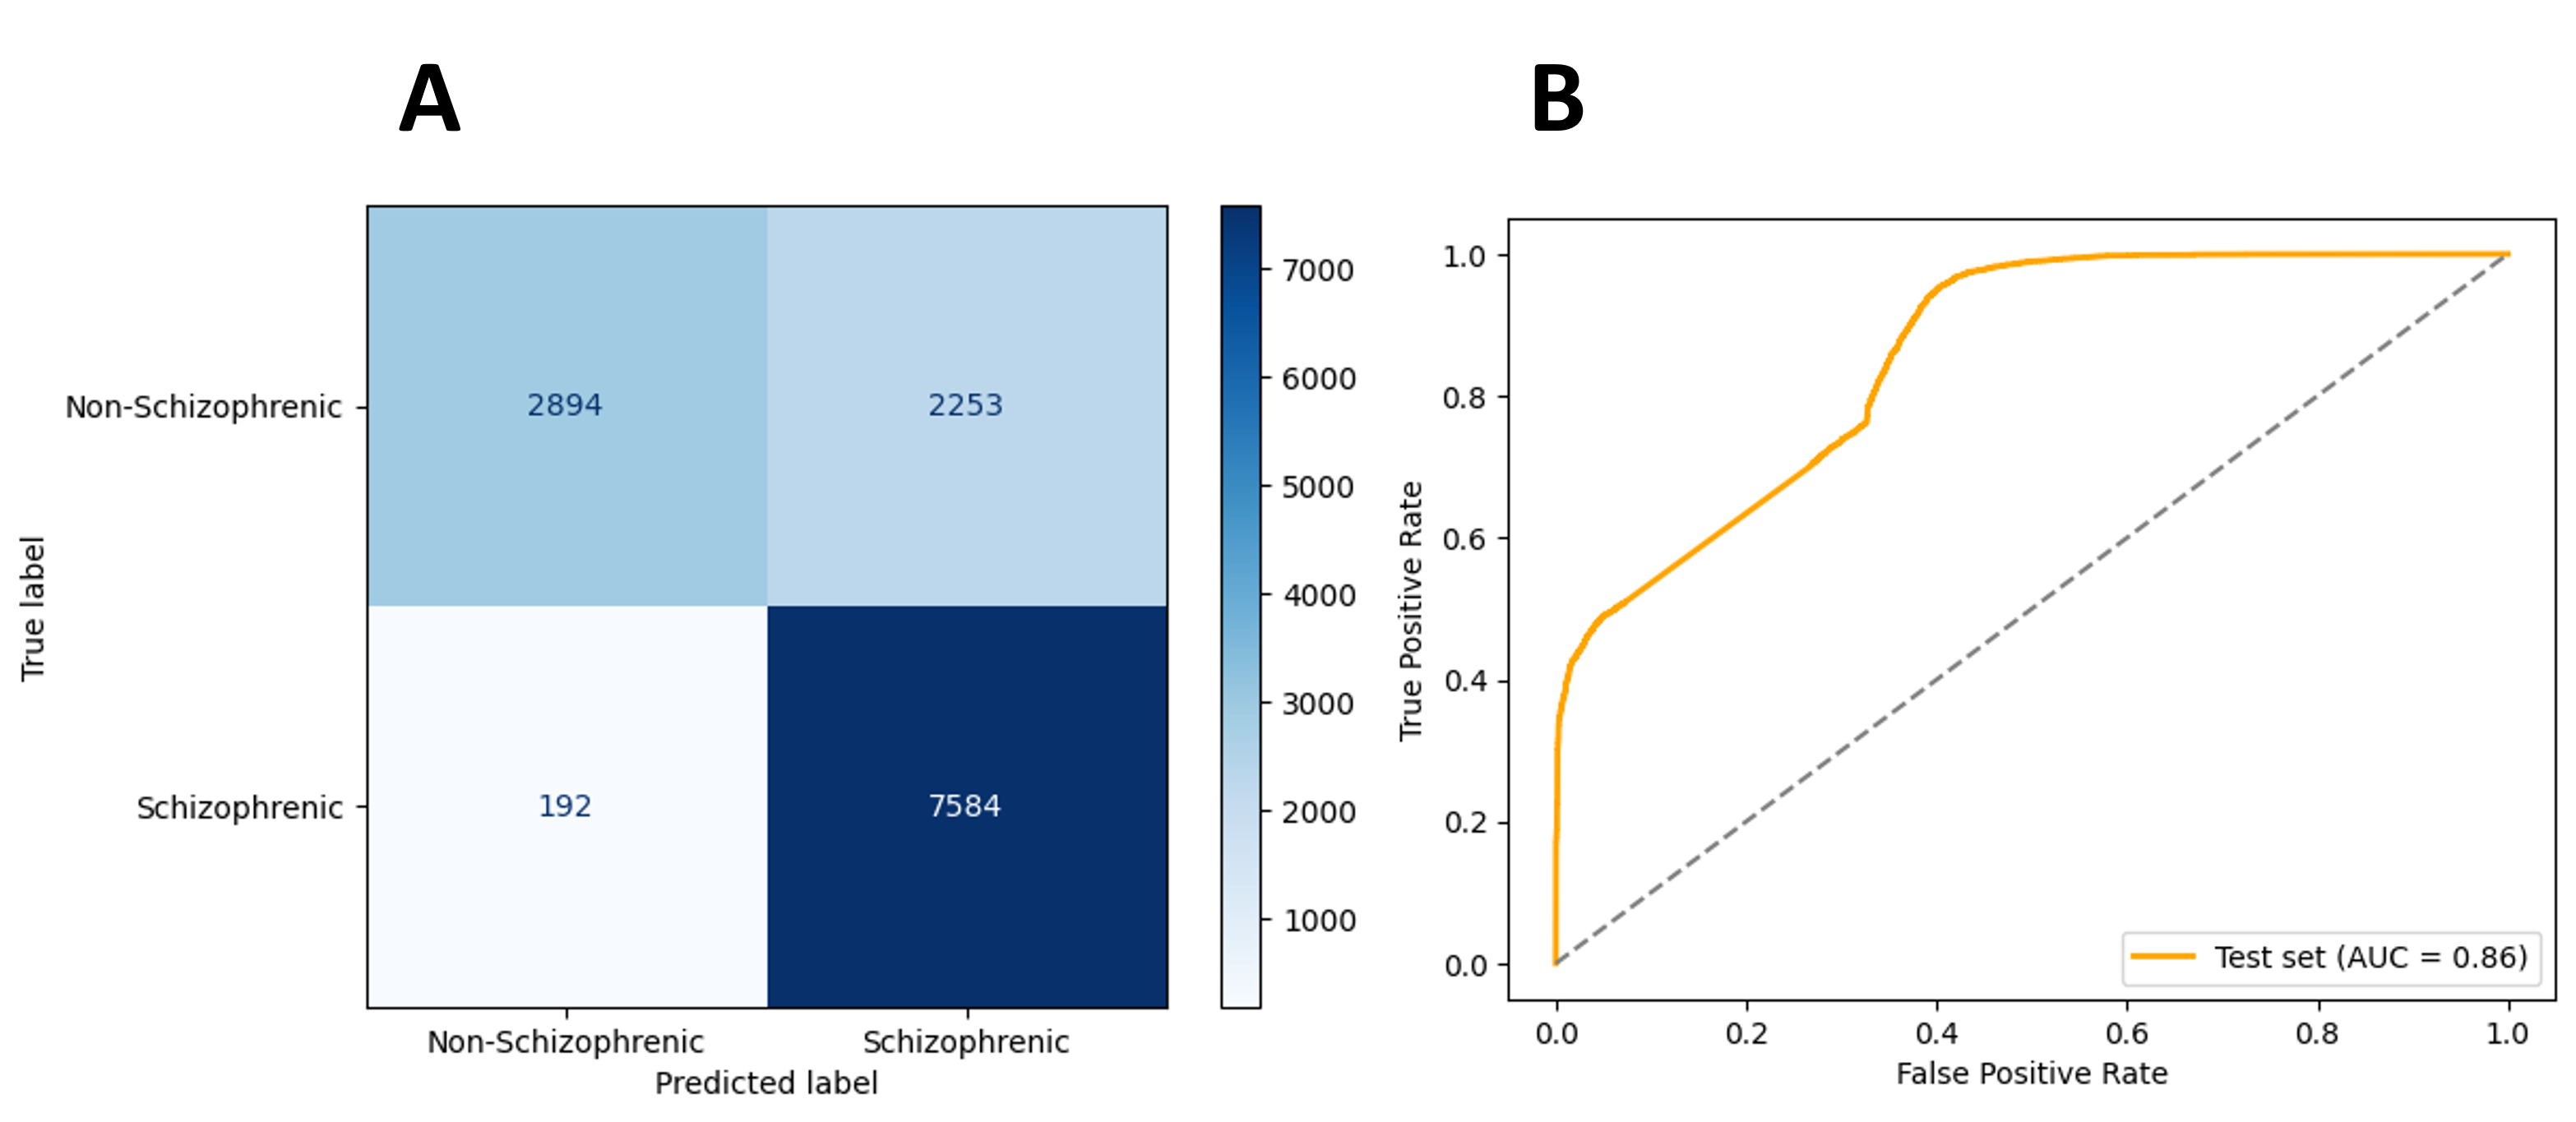
\includegraphics[width=0.8\textwidth]{./figs/eval_final_model.png} % 
    \caption{Preprocessing and augmentation steps: resampling + normalization + brain extraction + translation + rotation. Panel A: confusion matrix with recall of 0.98. Panel B: ROC curve with AUC of 0.86}\label{fig:eval_final_model}
\end{figure}

\begin{figure}
    \centering
    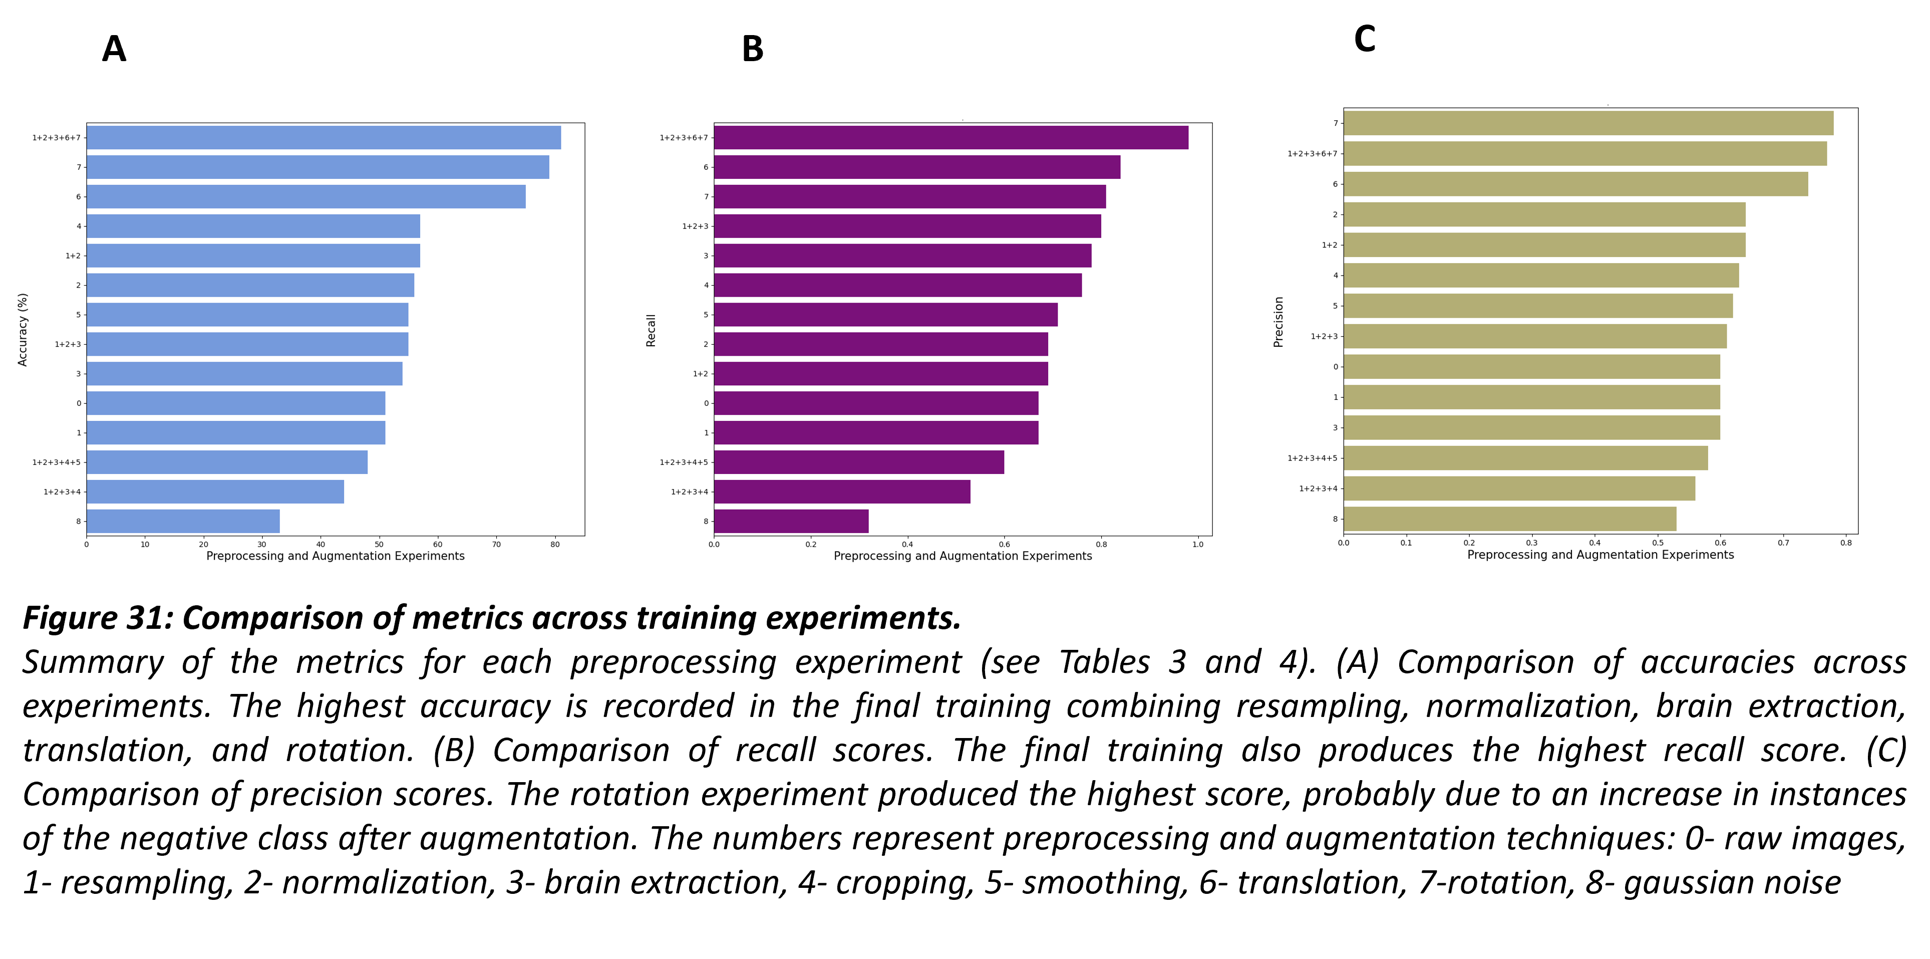
\includegraphics[width=0.8\textwidth]{./figs/model_metrics_comparison.png} % 
    \caption{Summary of the metrics for each preprocessing experiment. Panel A: comparison of accuracies across the experiments. The highest accuracy was recorded in the final experiment combining resampling, normalization, brain extraction, translation and rotation. Panel B: comparison of recall scores. The final experiment yielded the highest recall score. Panel C: comparison of precision scores. The rotation experiment produced the highest score, probably due to an increase in instances of the negative class after augmentation. The numbers along the y-axis represent preprocessing and augmentation scenarios: 0 --- raw images, 1 --- resampling, 2 --- normalization, 3 --- brain extraction, 4 --- cropping, 5 --- smoothing, 6 --- translation, 7 --- rotation, 8 --- Gaussian noise.}\label{fig:model_metrics_comparison}
\end{figure}


% Discussion
\section{Discussion}

This study investigated the effects of various preprocessing and data augmentation techniques on the classification performance of schizophrenia from structural MRI data. The results demonstrate that certain preprocessing steps, such as normalization, brain extraction, and cropping, can improve model performance when applied individually. However, combining these steps did not yield consistent improvements, suggesting that over-processing may distort the data and hinder the model's ability to generalize effectively.

Among the individual preprocessing techniques, normalization resulted in the most substantial performance improvement, enhancing accuracy to 56\% (9.8\% increase compared to baseline). This can be attributed to the equalization of feature contributions, which allowed the model to make more accurate predictions. Interestingly, this outcome contradicts the conventional understanding that normalizing medical images may flatten clinically significant differences in intensity. The effectiveness of this technique in this study highlights the importance of context when applying preprocessing methods to medical imaging.

Brain extraction, or skull stripping, while beneficial in other studies, had a moderate effect here, improving recall but slightly lowering accuracy. This suggests that removing non-brain tissues enhances the model's sensitivity to schizophrenia cases but may reduce precision, potentially due to the loss of relevant contextual information in the brain image. Cropping, on the other hand, demonstrated a clear advantage by improving accuracy and F1-score. By focusing on the brain region and reducing irrelevant background data, cropping effectively improved the signal-to-noise ratio, allowing the model to focus on clinically relevant features.

However, combining preprocessing steps often led to diminished performance, especially when all techniques were applied together. While the best performance was achieved with resampling, normalization, and brain extraction, adding further steps, such as cropping and smoothing, resulted in a performance drop, particularly in terms of accuracy and F1-score. This suggests that certain preprocessing steps, when combined, may interfere with each other, creating distortions that prevent the model from learning the most pertinent features of the data.

Regarding data augmentation, both translation and rotation significantly enhanced model performance, with translation improving recall and rotation achieving the highest accuracy and F1-score. These results align with the literature, where such transformations are often used to increase the diversity of the training data, helping the model generalize better to unseen samples. Gaussian noise, however, severely degraded performance, suggesting that it may obscure important features in the MRI images, leading to poorer model predictions.

The final training model, which combined the optimal preprocessing steps (resampling, normalization, and brain extraction) with translation and rotation (1+2+3+6+7), achieved the highest overall performance, with an accuracy of 81\%, recall of 0.98, and an F1-score of 0.86. This result demonstrates the effectiveness of combining well-selected preprocessing and augmentation techniques in enhancing classification performance. Notably, the final model's recall score suggests that it is highly sensitive to positive cases, which is crucial for medical applications where detecting true positives is a priority.

While preprocessing techniques like skull stripping, cropping, and smoothing have been shown to improve performance in various medical imaging tasks, the results in this study suggest that their effectiveness depends on the context and the combination of other preprocessing steps. Furthermore, the adverse effect of Gaussian noise indicates the need for careful consideration of the types of augmentation applied, as certain methods may introduce detrimental effects.

In contrast to some previous studies that have used more complex augmentation techniques, such as elastic deformations, this study focused on simpler methods, which proved to be more effective. Elastic deformations can sometimes introduce unrealistic and unnatural variations, leading to damage and noise that harm model performance~\cite{Mok2018}. The methods investigated in this study, particularly translation and rotation, were found to be effective in maintaining the integrity of the original images while enhancing model robustness.

Overall, this study highlights the importance of standardizing preprocessing and augmentation techniques in medical imaging, particularly for tasks like schizophrenia detection. The results suggest that the combination of multiple preprocessing steps should be approached with caution, as it may lead to diminishing returns or reduced model performance while a well-optimized combination of preprocessing and augmentation can significantly improve model performance. Further research is needed to explore additional augmentation strategies and evaluate their impact on model generalizability in larger and more diverse datasets.

%augmentation with the combination of shearing and salt-and-pepper noise addition is the least efficient approach for augmentation in improving classification performance 

% Discuss When Brain Extraction May Not Be Necessary

% Discuss Metrics for Each 2D Slice (Slice-wise Approach):


% Conclusion
\section{Conclusion}

This study examined the impact of preprocessing and data augmentation on schizophrenia classification from structural MRI images. The best preprocessing setup (resampling + normalization + brain extraction) improved performance (55\% accuracy, 0.69 F1-score), but excessive preprocessing did not yield further gains.

Data augmentation had a stronger effect, with rotation achieving the highest accuracy (79\%) and F1-score (0.80). The final model, trained with optimized preprocessing and augmentation, achieved the best overall performance (81\% accuracy, 0.98 recall), highlighting the value of spatial transformations.

The findings emphasize the importance of careful selection and application of preprocessing and augmentation methods in medical imaging tasks. The results underscore the need for a standardized preprocessing pipeline to enhance the reliability, reproducibility, and clinical applicability of machine learning models for schizophrenia detection.

Further work is needed to refine preprocessing pipelines and explore additional augmentation methods to improve the performance of ML-based schizophrenia diagnosis. Ultimately, this study contributes to the ongoing efforts to make ML-driven medical diagnostics more robust and applicable in real-world clinical settings.

% Formalities
%\section*{Acknowledgements}

%...

\subsection*{Author contributions}

\textbf{Conception}: Prosperity Oguama, Ilia Golub; \textbf{Data Acquisition}: Ilia Golub; \textbf{Preprocessing \& Data Augmentation}: Ilia Golub; \textbf{Model Building \& Testing}: Prosperity Oguama; \textbf{Drafting \& Editing}: Ilia Golub, Prosperity Oguama. All authors contributed to the study, read, revised and approved the final manuscript.

\subsection*{Data availability statement}
The data underlying this article is publicly available and accessible through \hyperlink{Schizconnect}{http://schizconnect.org/}.

\subsection*{Financial disclosure}

The authors report no financial disclosure.

\subsection*{Conflict of interest}

The authors declare no potential conflict of interests.

\renewcommand{\baselinestretch}{1.5}
%\singlespacing
%\renewcommand\bibname{Bibliography}
\bibliographystyle{abbrv} %abbrv
\phantomsection     % 
\cleardoublepage    % 
\bibliography{paper}

\end{document}